% !TeX spellcheck = en_US
% !TeX root = main.tex

\section{Website Implementation}
\subsection{Accessibility, Graceful Degradation \& Progressive Enhancement}
% What were the key things you learned from your Accessibility, Graceful Degradation and Progressive Enhancement group discussions?
% Write brief responses of your own to the guiding questions for these group discussions
% Rationalise why you've chosen to use JavaScript instead of HTML hyperlinks or CSS features of your website
% How has your website used a combination of HTML, CSS and JavaScript to great effect?

\subsubsection{Accessibility}
\begin{figure}
	\centering
	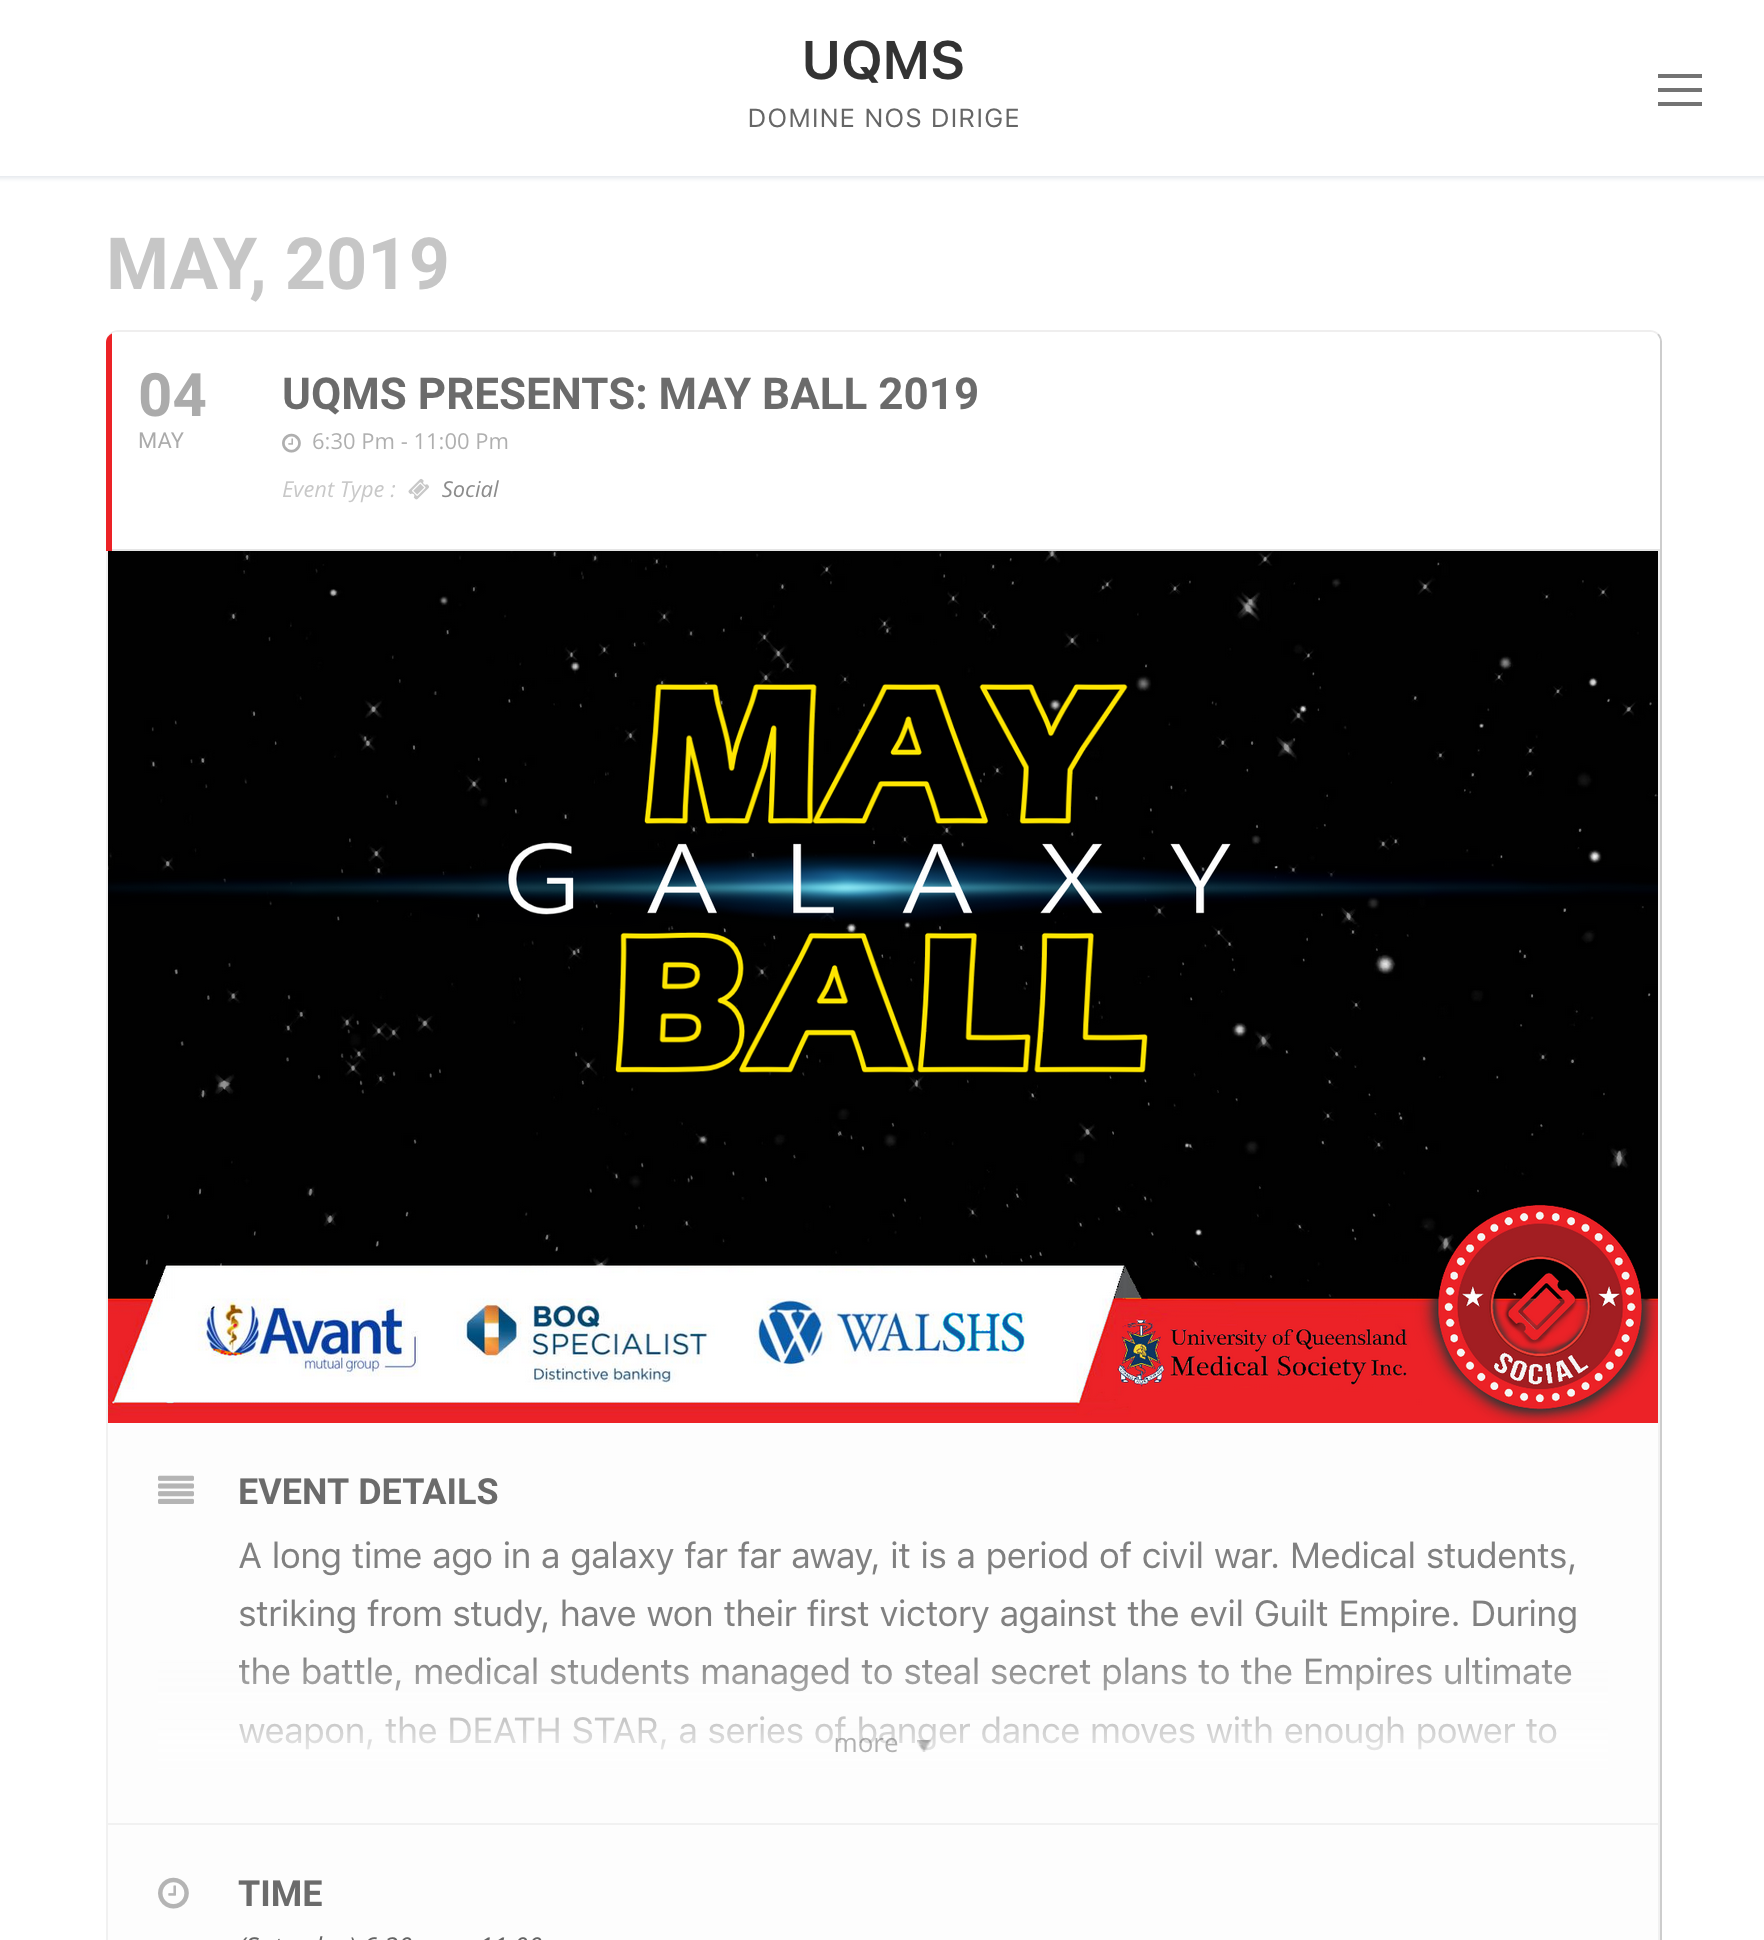
\includegraphics[width=0.7\linewidth]{mayball}
	\caption{Screenshot of the event page for the 2019 May Ball hosted by \gls{uqms}}\label{fig:uqms}
\end{figure}
All website should be accessible to their users and have support for people with impairments or a disadvantage. The \gls{wcag} outlines four key areas all websites should be assessed on and how these areas impact people and their use of the site. Figure~\ref{fig:uqms} shows a screenshot of the event page for the \gls{uqms} Ball in 2019, the accessibility of this site is as follows:
\begin{description}
	\item[Perceivable:] While all content is available upfront to the user, not all of the non-text content of the website has a text alternative. A lot of the images have not provided an \texttt{alt} attribute. However all of the content is presented visually in a simple one dimensional structure format, the choice in colours between the foreground and the background has resulted in a difficulty to view and read the content.
	\item[Operable:] The website is not operable purely from a keyboard, being able to view and read all of the content on the website requires the use of a mouse to expand the details. The navigation works as expected, allowing users to clearly and quickly identify where they are and being able to navigate to different pages easily through the menu.
	\item[Understandable:] The content is clearly sectioned and defined making it easy to read and understand what is being delivered. It follows a structure similar to other events pages and is clearly family upon opening.
	\item[Robust:] Upon inspecting the source of the website it is clear that the robustness of the website is lacking behind common web standards. An example is the clutter of div tags. With the lack of use of normal semantic \gls{html} tags and nesting content inside of \texttt{p} tags.
\end{description}


\subsubsection{Graceful Degradation}
\begin{figure}
	\centering
	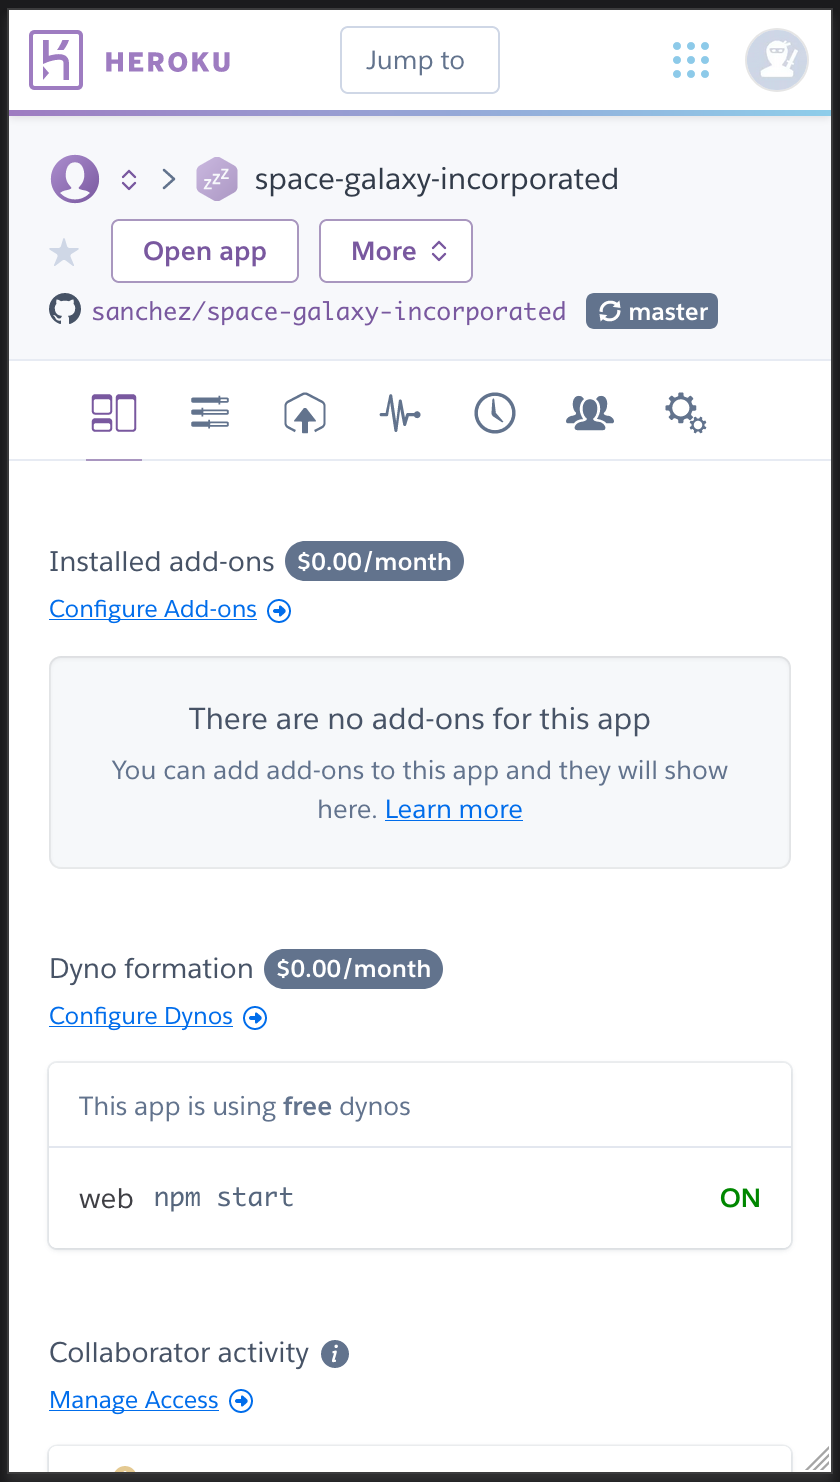
\includegraphics[width=0.3\linewidth]{heroku1}	
	\caption{Screenshot of the \gls{heroku} dashboard in a mobile view}\label{fig:heroku}
\end{figure}

An example of graceful degradation is the \gls{heroku} administrator dashboard. Figure~\ref{fig:heroku} shows the site in a mobile view, graceful degradation is applied here because the site is still usable, however some of the float controls have been wrapped around and not displayed as mobile friendly as possible. The ``Open App'' button could be collapsed into the ``More'' button and relabelled to represent a hamburger icon. The website overall is useful as a mobile application however, therefore the site gracefully degrades from desktop to mobile.

\subsubsection{Progressive Enhancement}
\begin{figure}
	\centering
	\subfloat[Mobile version of \gls{bootstrap}'s checkout]{
		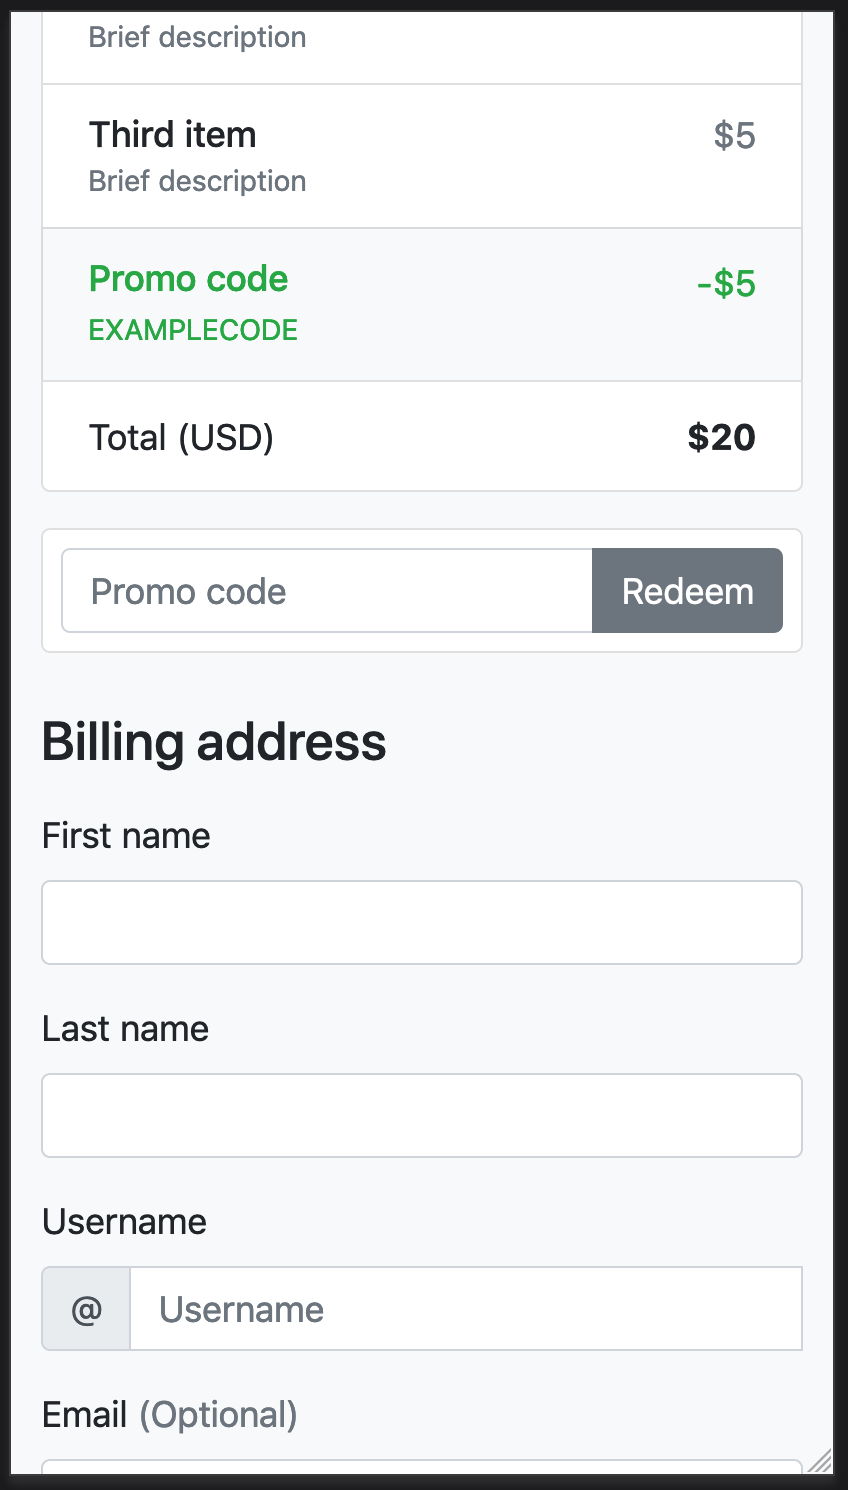
\includegraphics[width=0.3\textwidth]{bootstrap2}\label{fig:bootstrap:mobile}}
	\qquad
	\subfloat[Desktop version of \gls{bootstrap}'s checkout]{
		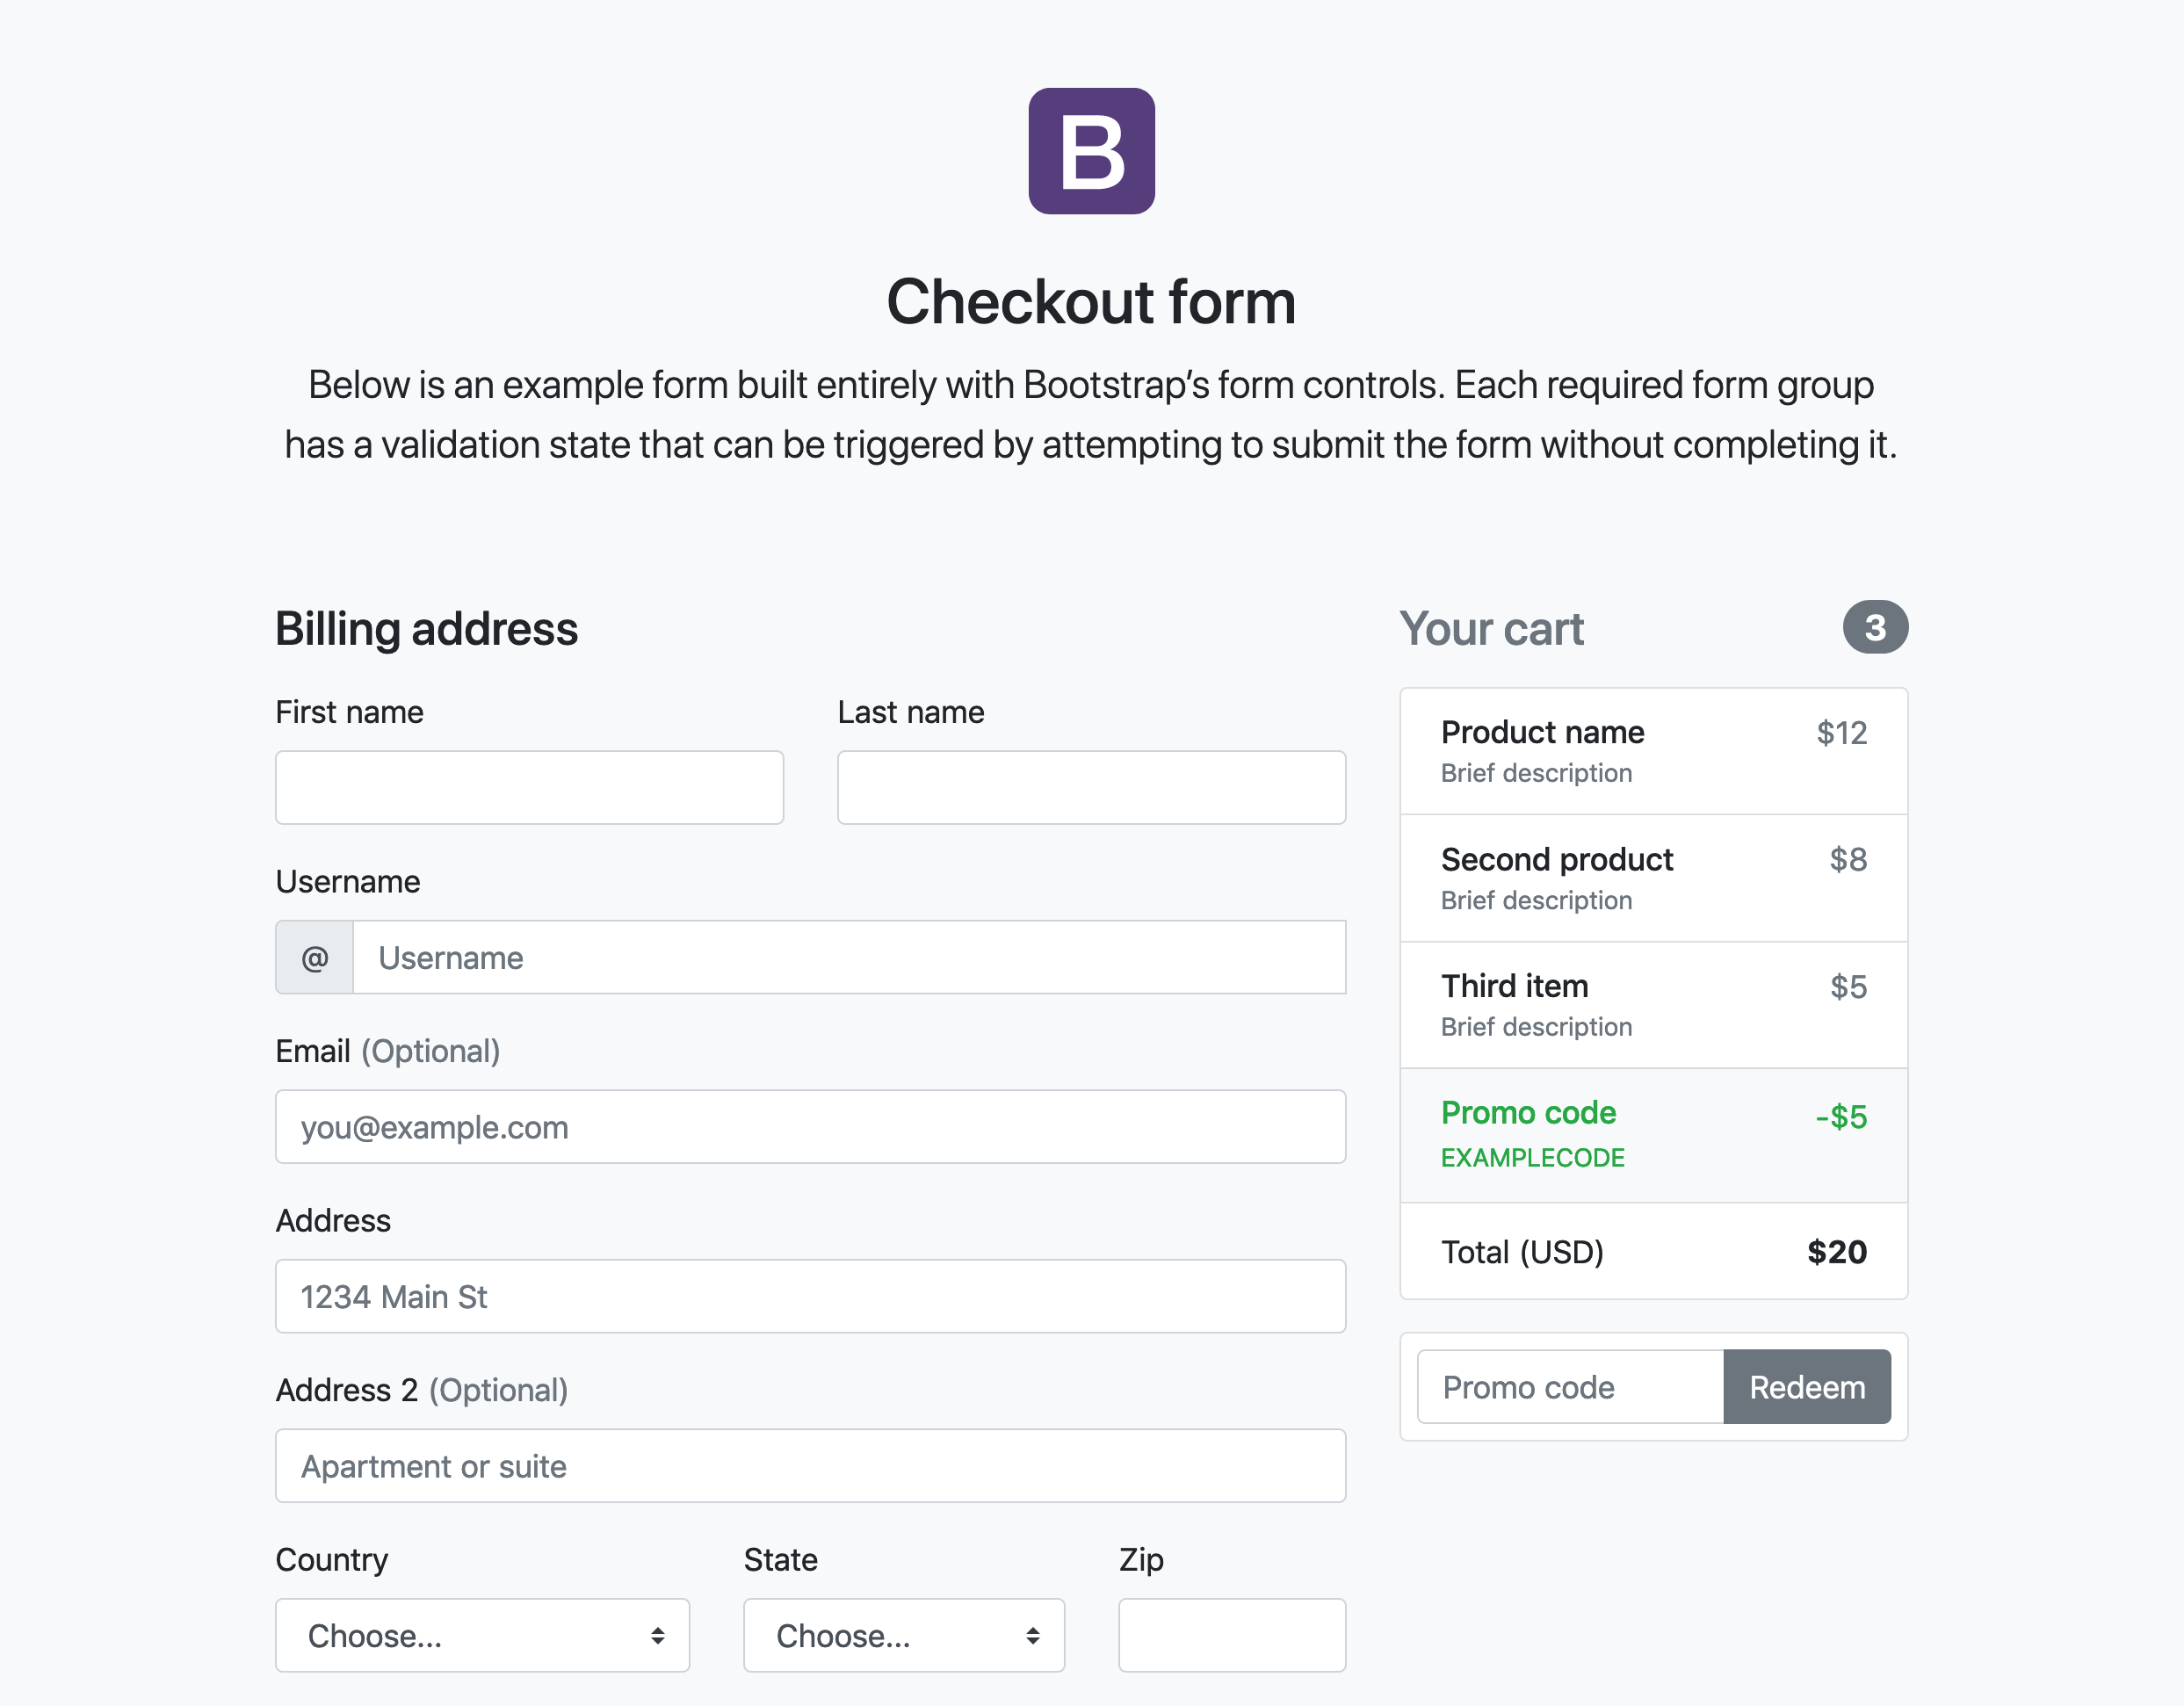
\includegraphics[width=0.6\textwidth]{bootstrap3}\label{fig:bootstrap:desktop}}
	\caption{Screenshots of \gls{bootstrap}'s example checkout page}\label{fig:bootstrap}
\end{figure}

\gls{bootstrap} is a perfect example of progressive enhancement, because the entire framework is around mobile-first design. Mobile-first design forces the designer to design the website with mobile in mind first and then once the site is designed mobile it can be scaled up to desktop with extra features being added and removed based on the screen size. Figure~\ref{fig:bootstrap} shows a comparison of the website between the mobile and desktop.\\\\
As seen in Figure~\ref{fig:bootstrap:mobile} the checkout list appears in the list however in Figure~\ref{fig:bootstrap:mobile} the list appears on the right side of the page. This design choice means the user is presented with the most important content first in mobile view but following common checkout design patterns in desktop view. This is achieved using media queries with respect to the window size, allowing for the window to be flexible and the mobile page is presented if the desktop screen size is too small.\\\\
Another notable difference is in the layout of the form for the billing address. In the desktop there are multiple columns of fields, but on the mobile version everything is one dimensional (all the fields flow down the page). This is achieved using both flexboxes to define the way content should flow in the page, and media queries to define the size of the columns and content inside the columns.

\subsubsection{Reflection}
It is clear that a direction of either degradation or enhancement is needed to be chosen. Since the website is primarily focussed at users on a computer (since \gls{git} is desktop only tool), the main focus will be on desktop devices and the website will gracefully degrade to support mobile devices. The accessibility of the website can be reinforced by picking more contrasting colours to help with identification of sections, and the use of more semantic \gls{html} can help improve the robustness.

\subsection{Security \& Privacy}
% What were the key things you learned from your Security \& Privacy group discussions?
% Write brief responses of your own to the guiding questions for these group discussions
\subsubsection{Security}
\begin{figure}
	\centering
	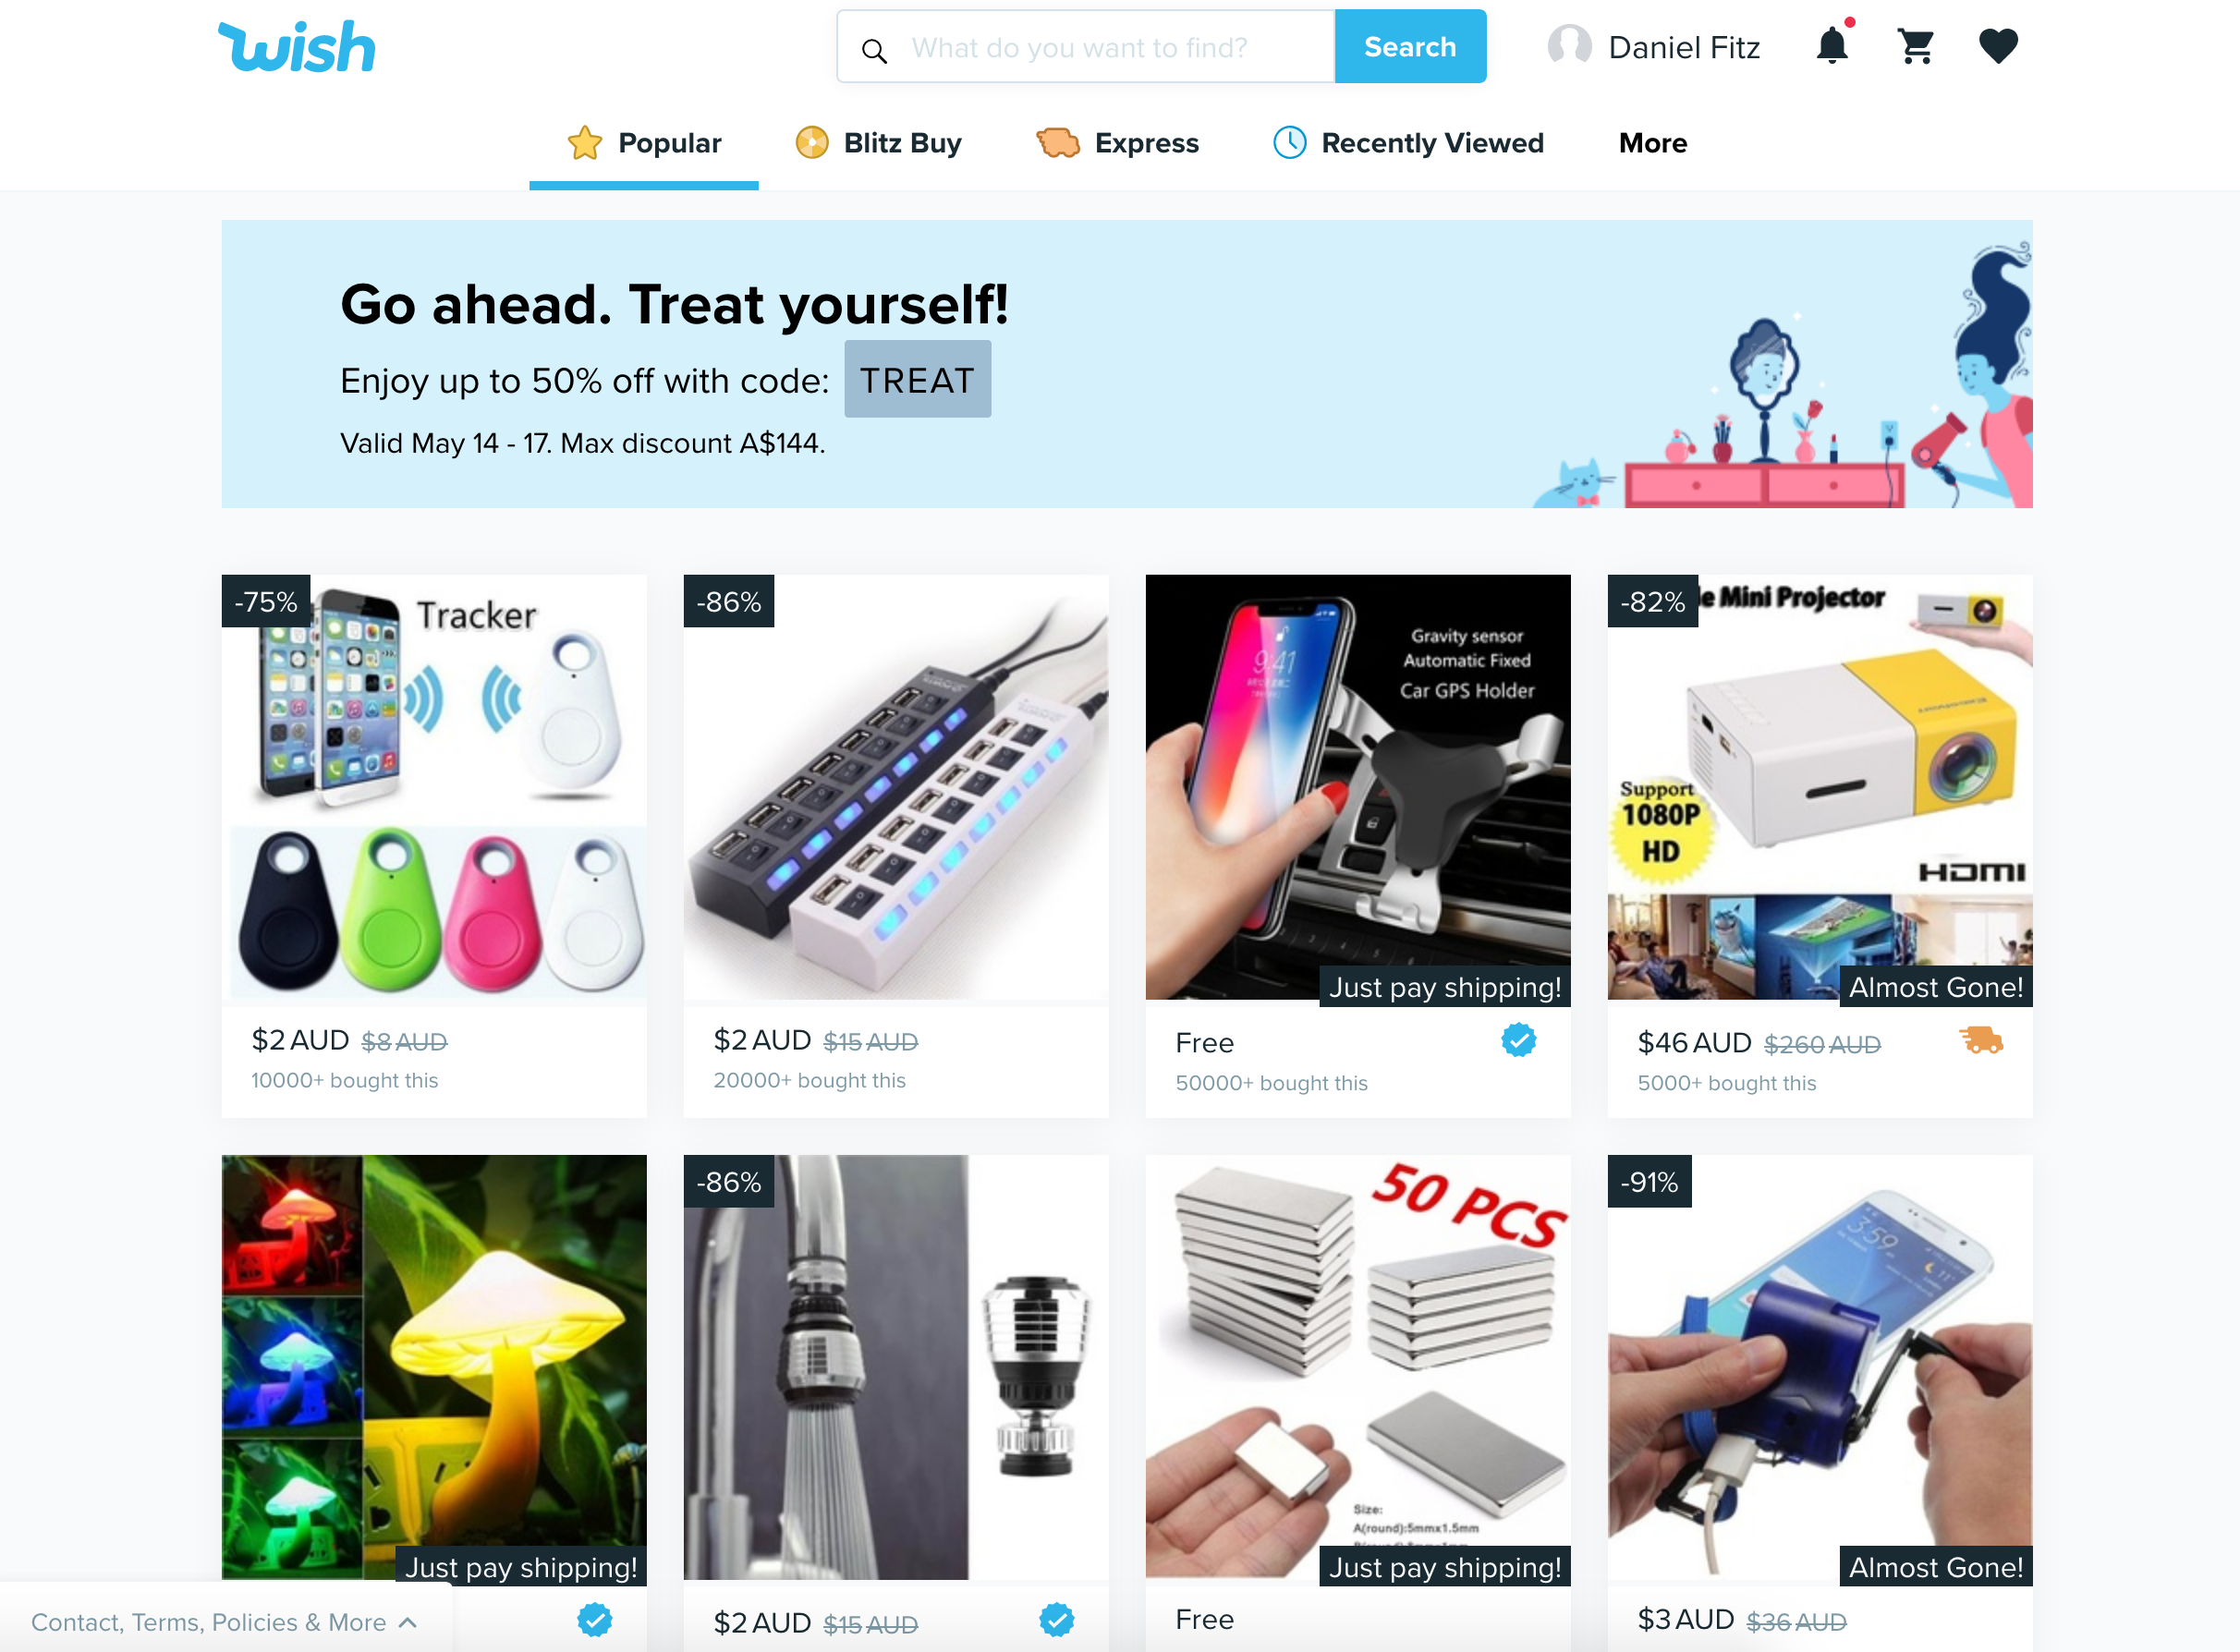
\includegraphics[width=0.8\linewidth]{wish}
	\caption{Screenshot of the homepage of a Wish.com site}\label{fig:wish}
\end{figure}
Security plays a massive role in modern web consumption, especially with ecommerce sites such as Wish.com. Wish.com is a site for buying and selling items online at really cheap prices. Figure~\ref{fig:wish} shows a screenshot of the landing page of Wish.com, some initial security threats are alerted when evaluating this website:
\begin{itemize}
	\item A lot of the items are so cheap it can sort of feel like a quick and dirty scam
	\item There is little to no descriptions about the items for sale
	\item The images of the items do not look representative of the real items
	\item The site attempted to run Flash scripts
	\subitem Flash has long been considered a threat to web security due to the access it has to the underlying \gls{os}	
\end{itemize}
While these are some strong security threats, Wish.com also has some good security initiatives in place to protect itself and the users:
\begin{itemize}
	\item The website is clean and unclustered
	\item There is a review system and a seller review system
	\item Purchases can be made using \gls{paypal}
	\item The site forces the use of \gls{https}
	\subitem The certificate is however verified and assigned to GoDaddy, which a relationship is not mentioned on the site anywhere	
\end{itemize}

\subsubsection{Privacy}
\begin{figure}[H]
	\centering
	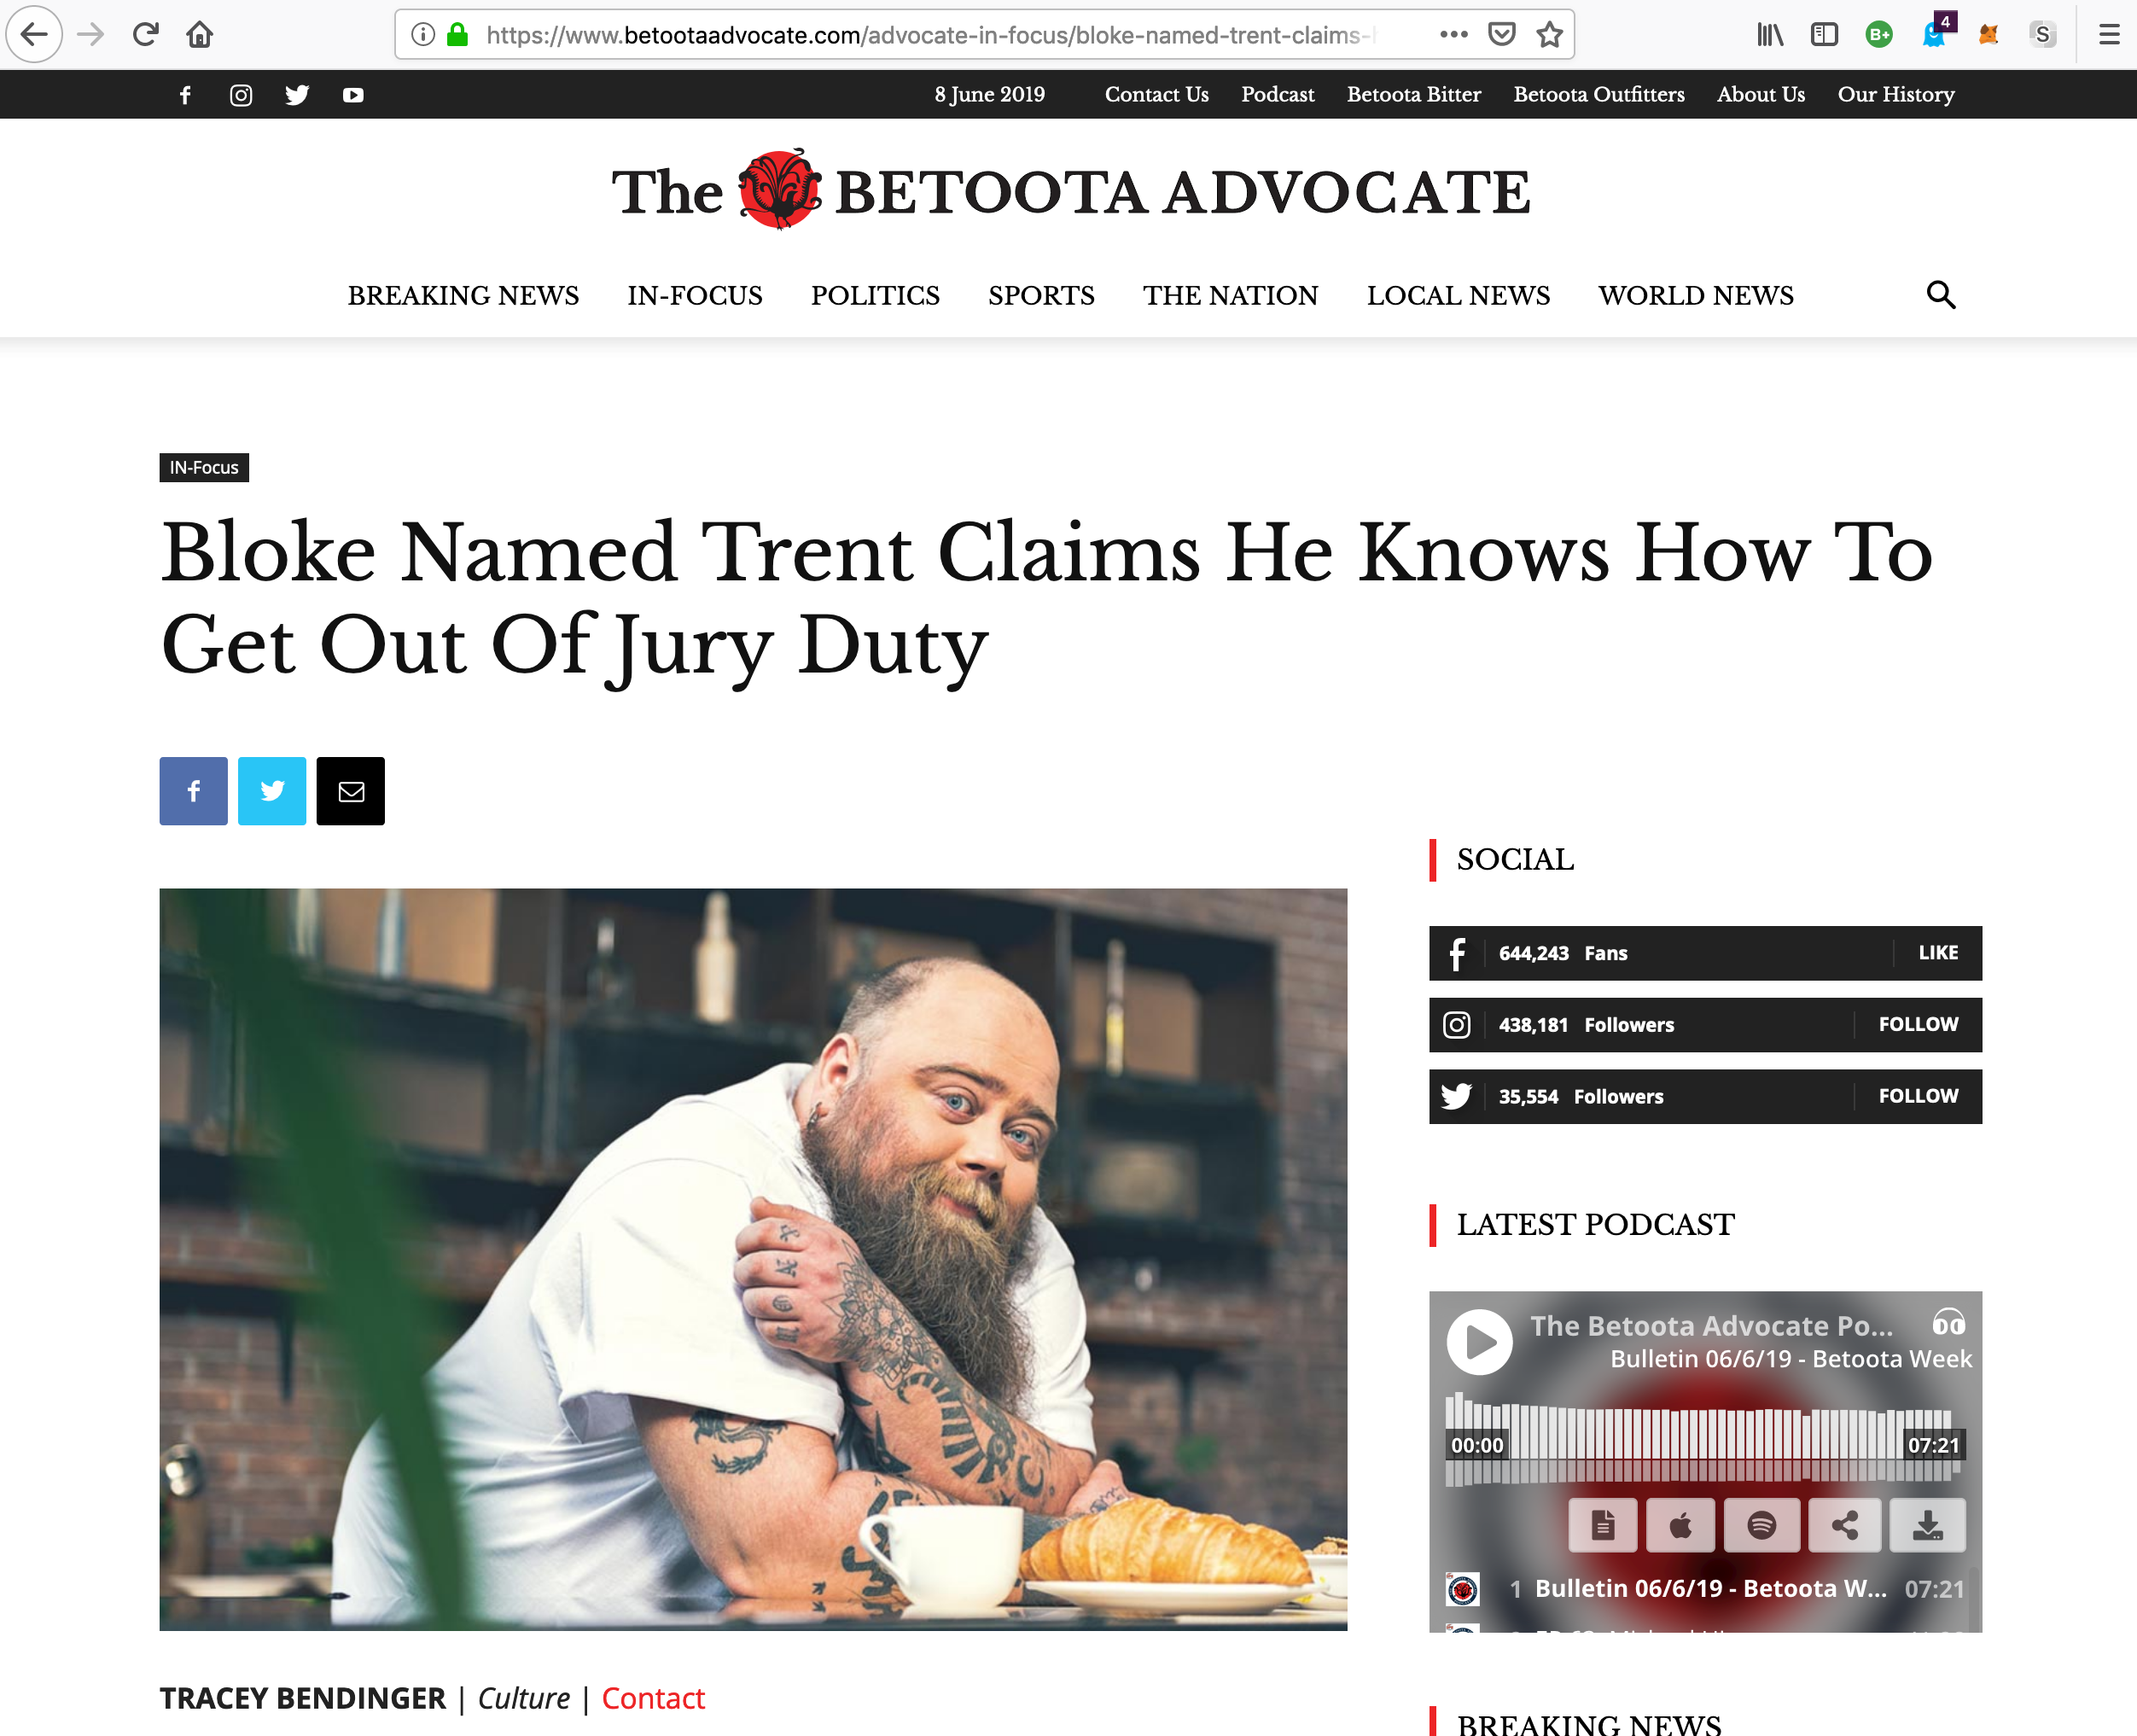
\includegraphics[width=0.7\linewidth]{betoota}
	\caption{Screenshot of a news article on The Betoota Advocate}\label{fig:betoota}
\end{figure}
User privacy is important to not only be aware of but to also respect too. The Betoota Advocate is a popular website providing news articles to users, news article providers benefit greatly from trackers and advertisements. However Betoota is different because Ghostery has alerted that there are no advertisements and only three trackers used in the article being observed (Figure~\ref{fig:betoota}). On top of the minimal trackers and advertisements, Betoota also has minimal cookies in use (10 cookies in total) most of which are related to third-party tools or services the site uses.

\subsection{Hi-Fi User Testing}
% Reflect on the success of the Hi-Fi User Testing design activity you did in Week 13
% Include the testing plan you developed for the activity
% Include photos you took of the activity running
% What feedback did you get and how did it inform your final product?
For the Hi-Fi User Testing task there were five main instructions requested from the user to complete during the session:
\begin{enumerate}
	\item Learn the basics of Git
	\subitem Observe the speed at which the user consumes the knowledge on the homepage
	\item Access the Quizzes page
	\subitem Observe if they look for a link on the homepage or in the navigation bar
	\item Find an advanced command
	\subitem Observe if they scroll through the page and look for an advanced looking command or jump to the references page
	\item Complete the first question involving the terminal sandbox
	\subitem Observe how the user interacts with the sandbox, is there clear direction to their actions
	\item Create a branch in the terminal sandbox
	\subitem Observe if the user switches back to the main tutorial to look for commands
\end{enumerate}
Upon initial observations it became clear that users were unable to realise the site could be scrolled and the homepage contained content past the first screen. This set back placed a lot of users in a place of confusion and frustration already. Therefore when they realised they could scroll they really quickly skimmed through all the content without properly observing the information and reading.\\\\
Access the quizzes page was done primarily through the use of the navigation bar, with only one user looking at the bottom of the page for a quiz link after reading the content.\\\\
The advanced command however, most users thought an advanced command was a command covered on the page and had no idea there were more commands hidden in the references page.\\\\
Both tasks involving the the \gls{git} sandbox resulted in the users not being able to understand how to use the sandbox and not knowing what commands to use. Some of the users also noted they had no idea the text in the grey boxes were commands that could be run in the sandbox.

\subsubsection{Reflection}
Upon receiving this feedback it was clear some adjustments were required to get the product up a standard that is usable for users. Some minor changes are needed to be made to fix the issues people had with the Hi-Fi test:
\begin{itemize}
	\item Add an arrow or some indication on the first screen to inform users that they can scroll down. Also make this action interactive so that if the user clicks on it they will be moved down to the next section.
	\item Make the side menu more noticeable via the use of some animation, most users were not aware it could be used or even existed.
	\item Add a final paragraph that links to the other pages as an indicator for the next steps the user can take.
	\item Add some tooltips to both the command boxes and the \gls{git} sandbox to help the user understand what the content is for and how to use it.
\end{itemize}





